% A LaTeX template for ARTICLE version of the MSc Thesis submissions to 
% Politecnico di Milano (PoliMi) - School of Industrial and Information Engineering
%
% S. Bonetti, A. Gruttadauria, G. Mescolini, A. Zingaro
% e-mail: template-tesi-ingind@polimi.it
%
% Last Revision: October 2021
%
% Copyright 2021 Politecnico di Milano, Italy. Inc. NC-BY

\documentclass[11pt,a4paper]{article} 

%------------------------------------------------------------------------------
%	REQUIRED PACKAGES AND  CONFIGURATIONS
%------------------------------------------------------------------------------
% PACKAGES FOR TITLES
\usepackage{titlesec}
\usepackage{color}

% PACKAGES FOR LANGUAGE AND FONT
\usepackage[utf8]{inputenc}
\usepackage[english]{babel}
\usepackage[T1]{fontenc} % Font encoding

% PACKAGES FOR IMAGES
\usepackage{graphicx}
\usepackage[utf8]{inputenc}
\graphicspath{{Images/}}
\usepackage{eso-pic} % For the background picture on the title page
\usepackage{subfig} % Numbered and caption subfigures using \subfloat
\usepackage{caption} % Coloured captions
\usepackage{transparent}

% STANDARD MATH PACKAGES
\usepackage{amsmath}
\usepackage{amsthm}
\usepackage{bm}
\usepackage[overload]{empheq}  % For braced-style systems of equations

% PACKAGES FOR TABLES
\usepackage{tabularx}
\usepackage{longtable} % tables that can span several pages
\usepackage{colortbl}

% PACKAGES FOR ALGORITHMS (PSEUDO-CODE)
\usepackage{algorithm}
\usepackage{algorithmic}

% PACKAGES FOR REFERENCES & BIBLIOGRAPHY
\usepackage[colorlinks=true,linkcolor=black,anchorcolor=black,citecolor=black,filecolor=black,menucolor=black,runcolor=black,urlcolor=black]{hyperref} % Adds clickable links at references
\usepackage{cleveref}
\usepackage[square, numbers, sort&compress]{natbib} % Square brackets, citing references with numbers, citations sorted by appearance in the text and compressed
\bibliographystyle{plain} % You may use a different style adapted to your field

% PACKAGES FOR THE APPENDIX
\usepackage{appendix}

% PACKAGES FOR ITEMIZE & ENUMERATES 
\usepackage{enumitem}

% OTHER PACKAGES
\usepackage{amsthm,thmtools,xcolor} % Coloured "Theorem"
\usepackage{comment} % Comment part of code
\usepackage{fancyhdr} % Fancy headers and footers
\usepackage{lipsum} % Insert dummy text
\usepackage{tcolorbox} % Create coloured boxes (e.g. the one for the key-words)
\usepackage{amsmath}
\usepackage{amssymb}

%-------------------------------------------------------------------------
%	NEW COMMANDS DEFINED
%-------------------------------------------------------------------------
% EXAMPLES OF NEW COMMANDS -> here you see how to define new commands
\newcommand{\bea}{\begin{eqnarray}} % Shortcut for equation arrays
\newcommand{\eea}{\end{eqnarray}}
\newcommand{\e}[1]{\times 10^{#1}}  % Powers of 10 notation
\newcommand{\mathbbm}[1]{\text{\usefont{U}{bbm}{m}{n}#1}} % From mathbbm.sty
\newcommand{\pdev}[2]{\frac{\partial#1}{\partial#2}}
% NB: you can also override some existing commands with the keyword \renewcommand

%----------------------------------------------------------------------------
%	ADD YOUR PACKAGES (be careful of package interaction)
%----------------------------------------------------------------------------


%----------------------------------------------------------------------------
%	ADD YOUR DEFINITIONS AND COMMANDS (be careful of existing commands)
%----------------------------------------------------------------------------


% Do not change Configuration_files/config.tex file unless you really know what you are doing. 
% This file ends the configuration procedures (e.g. customizing commands, definition of new commands)
% Configuration package
\usepackage[bottom=2.0cm,top=2.0cm,left=2.0cm,right=2.0cm]{geometry}
\raggedbottom 

% Create color bluePoli (-> manuale grafica coordinata:  https://www.polimi.it/fileadmin/user_upload/il_Politecnico/grafica-coordinata/2015_05_11_46xy_manuale_grafica_coordinata.pdf)
\definecolor{bluePoli}{cmyk}{0.4,0.1,0,0.4}

% Custom theorem environments
\declaretheoremstyle[
  headfont=\color{bluePoli}\normalfont\bfseries,
  bodyfont=\color{black}\normalfont\itshape,
]{colored}

\captionsetup[figure]{labelfont={color=bluePoli}} % Set colour of the captions
\captionsetup[table]{labelfont={color=bluePoli}} % Set colour of the captions
\captionsetup[algorithm]{labelfont={color=bluePoli}} % Set colour of the captions

\theoremstyle{colored}
\newtheorem{theorem}{Theorem}[section]
\newtheorem{proposition}{Proposition}[section]

% Enhances the features of the standard "table" and "tabular" environments.
\newcommand\T{\rule{0pt}{2.6ex}}
\newcommand\B{\rule[-1.2ex]{0pt}{0pt}}

% Algorithm description
\newcounter{algsubstate}
\renewcommand{\thealgsubstate}{\alph{algsubstate}}
\newenvironment{algsubstates}{
    \setcounter{algsubstate}{0}%
    \renewcommand{\STATE}{%
    \stepcounter{algsubstate}%
    \Statex {\small\thealgsubstate:}\space}
    }{}
    
% Custom theorem environment
\newcolumntype{L}[1]{>{\raggedright\let\newline\\\arraybackslash\hspace{0pt}}m{#1}}
\newcolumntype{C}[1]{>{\centering\let\newline\\\arraybackslash\hspace{0pt}}m{#1}}
\newcolumntype{R}[1]{>{\raggedleft\let\newline\\\arraybackslash\hspace{0pt}}m{#1}}

% Custom itemize environment
\setlist[itemize,1]{label=$\bullet$}
\setlist[itemize,2]{label=$\circ$}
\setlist[itemize,3]{label=$-$}
\setlist{nosep}

% Create command for background pic
\newcommand\BackgroundPic{% Adding background picture
	\put(237,365){
	    \parbox[b][\paperheight]{\paperwidth}{%
	    \vfill
		\centering
		\transparent{0.4}
		
\includegraphics[width=0.44\paperwidth]{raggiera_polimi.eps}%
		\vfill}
		}
}

% Set indentation
\setlength\parindent{0pt}

% Custom title commands
\titleformat{\section}
{\color{bluePoli}\normalfont\Large\bfseries}
{\color{bluePoli}\thesection.}{1em}{}
\titlespacing*{\section}
{0pt}{3.3ex}{3.3ex}

\titleformat{\subsection}
{\color{bluePoli}\normalfont\large\bfseries}
{\color{bluePoli}\thesubsection.}{1em}{}
\titlespacing*{\subsection}
{0pt}{3.3ex}{3.3ex}

% Custom headers and footers
\pagestyle{fancy}
\fancyhf{}
      
\fancyfoot{}
\fancyfoot[C]{\thepage} % page
\renewcommand{\headrulewidth}{0mm} % headrule width
\renewcommand{\footrulewidth}{0mm} % footrule width

\makeatletter
\patchcmd{\headrule}{\hrule}{\color{black}\hrule}{}{} % headrule
\patchcmd{\footrule}{\hrule}{\color{black}\hrule}{}{} % footrule
\makeatother

% Insert here the info that will be displayed into your Title page 
% -> title of your work
\renewcommand{\title}{Randomized Linear Algebra and its Applications}
% -> author name and surname
\renewcommand{\author}{Jasmin Spinetto, Peng Rao, Anna Paola Izzo, Cao Wu, Jiali Claudo Haung}
% -> MSc course
\newcommand{\course}{High Performance Computing Engineering - Advanced Methods for Scientific Computing}
% -> advisor name and surname
\newcommand{\advisor}{Prof. Luca Formaggia}
% IF AND ONLY IF you need to modify the co-supervisors you also have to modify the file Configuration_files/title_page.tex (ONLY where it is marked)
%\newcommand{\firstcoadvisor}{Name Surname} % insert if any otherwise comment
% -> author ID
\newcommand{\ID}{\\10734813, 11022931, ..., ..., ...}
% -> academic year
\newcommand{\YEAR}{2024-2025}
% -> abstract (only in English)
\renewcommand{\abstract}{Here goes the Abstract in English of your thesis (in article format)
followed by a list of keywords.
The Abstract is a concise summary of the content of the thesis (single page of text)
and a guide to the most important contributions included in your thesis.
The Abstract is the very last thing you write.
It should be a self-contained text and should be clear
to someone who hasn't (yet) read the whole manuscript.
The Abstract should contain the answers to the main research questions
that have been addressed in your thesis.
It needs to summarize the motivations and the adopted approach as well as
the findings of your work and their relevance and impact.
The Abstract is the part appearing in the record of your thesis inside POLITesi,
the Digital Archive of PhD and Master Theses (Laurea Magistrale) of Politecnico di Milano.
The Abstract will be followed by a list of four to six keywords.
Keywords are a tool to help indexers and search engines to find relevant documents.
To be relevant and effective, keywords must be chosen carefully.
They should represent the content of your work and be specific to your field or sub-field.
Keywords may be a single word or two to four words. }

% -> key-words (only in English)
\newcommand{\keywords}{Randomized Linear Algebra, RandomizedSVD, CUR Decomposition}

%-------------------------------------------------------------------------
%	BEGIN OF YOUR DOCUMENT
%-------------------------------------------------------------------------
\begin{document}

%-----------------------------------------------------------------------------
% TITLE PAGE
%-----------------------------------------------------------------------------
% Do not change Configuration_files/TitlePage.tex (Modify it IF AND ONLY IF you need to add or delete the Co-advisors)
% This file creates the Title Page of the document
% DO NOT REMOVE SPACES BETWEEN LINES!

\AddToShipoutPicture*{\BackgroundPic}

\hspace{-0.6cm}
\includegraphics[width=0.6\textwidth]{logo_polimi_ing_indinf.eps}

\vspace{-1mm}
\Large{\textbf{\color{bluePoli}{\title}}}\\

\vspace{-0.2cm}
\fontsize{0.3cm}{0.5cm}\selectfont \bfseries \textsc{\color{bluePoli} \course}\\

\vspace{-0.2cm}
\normalfont{\textbf{\author, \ID}}

\small \normalfont

\vspace{11pt}

\centerline{\rule{1.0\textwidth}{0.4pt}}

\begin{center}
\begin{minipage}[t]{.24\textwidth}
\begin{minipage}{.90\textwidth}
\noindent
\scriptsize{\textbf{Advisor:}} \\
\advisor \\
\\
% \textbf{Co-advisors:} \\ % leave it if any co-advisor otherwise comment
% \firstcoadvisor \\ % leave it if any co-advisor otherwise comment
% \secondcoadvisor \\ % leave it if you have more that one co-advisor otherwise comment (if you have more than two co-advisors just copy&paste this line writing \thirdcoadvisor, \fourthcoadvisor, ecc. (REMEMBER to modify also the main.txt)
\\ % leave it if any co-advisor otherwise comment
\textbf{Academic year:} \\
\YEAR \\
\\
\end{minipage}
\end{minipage}% This must go next to `\end{minipage}`
\begin{minipage}{.74\textwidth}
\noindent \textbf{\color{bluePoli} Abstract:} {\abstract}
\end{minipage}
\end{center}

\vspace{15pt}

\begin{tcolorbox}[arc=0pt, boxrule=0pt, colback=bluePoli!60, width=\textwidth, colupper=white]
    \textbf{Key-words:} \keywords
\end{tcolorbox}

\vspace{12pt}

%-----------------------------------------------------------------------------
% INTRODUCTION
%-----------------------------------------------------------------------------
\section{Introduction}
This project is a C++ implementation of the Randomized Singular Value Decomposition (rSVD) algorithm. We only used the matrix operations of the \texttt{Eigen} library to implement our algorithm. We do some benchmarks to compare the performance of our implementation with the Eigen library, the result indicates that our implementation can enhance the performance of handling large or sparse matrices.

We have already implemented the following algorithms:

\begin{itemize}
    \item QR factorization using Given's rotation: \texttt{GivensRotation}
    \item Basic SVD using Power Method: \texttt{PowerMethod}
    \item Randomized singular value decomposition: \texttt{RandomizedSVD}
\end{itemize}

Figure \ref{fig:speedup} shows the speedup of our implementation compared to \texttt{BDCSVD} the \texttt{Eigen} library. The speedup is calculated as the ratio of the time taken by the Eigen library to the time taken by our implementation.

\begin{figure}[H]
    \centering
    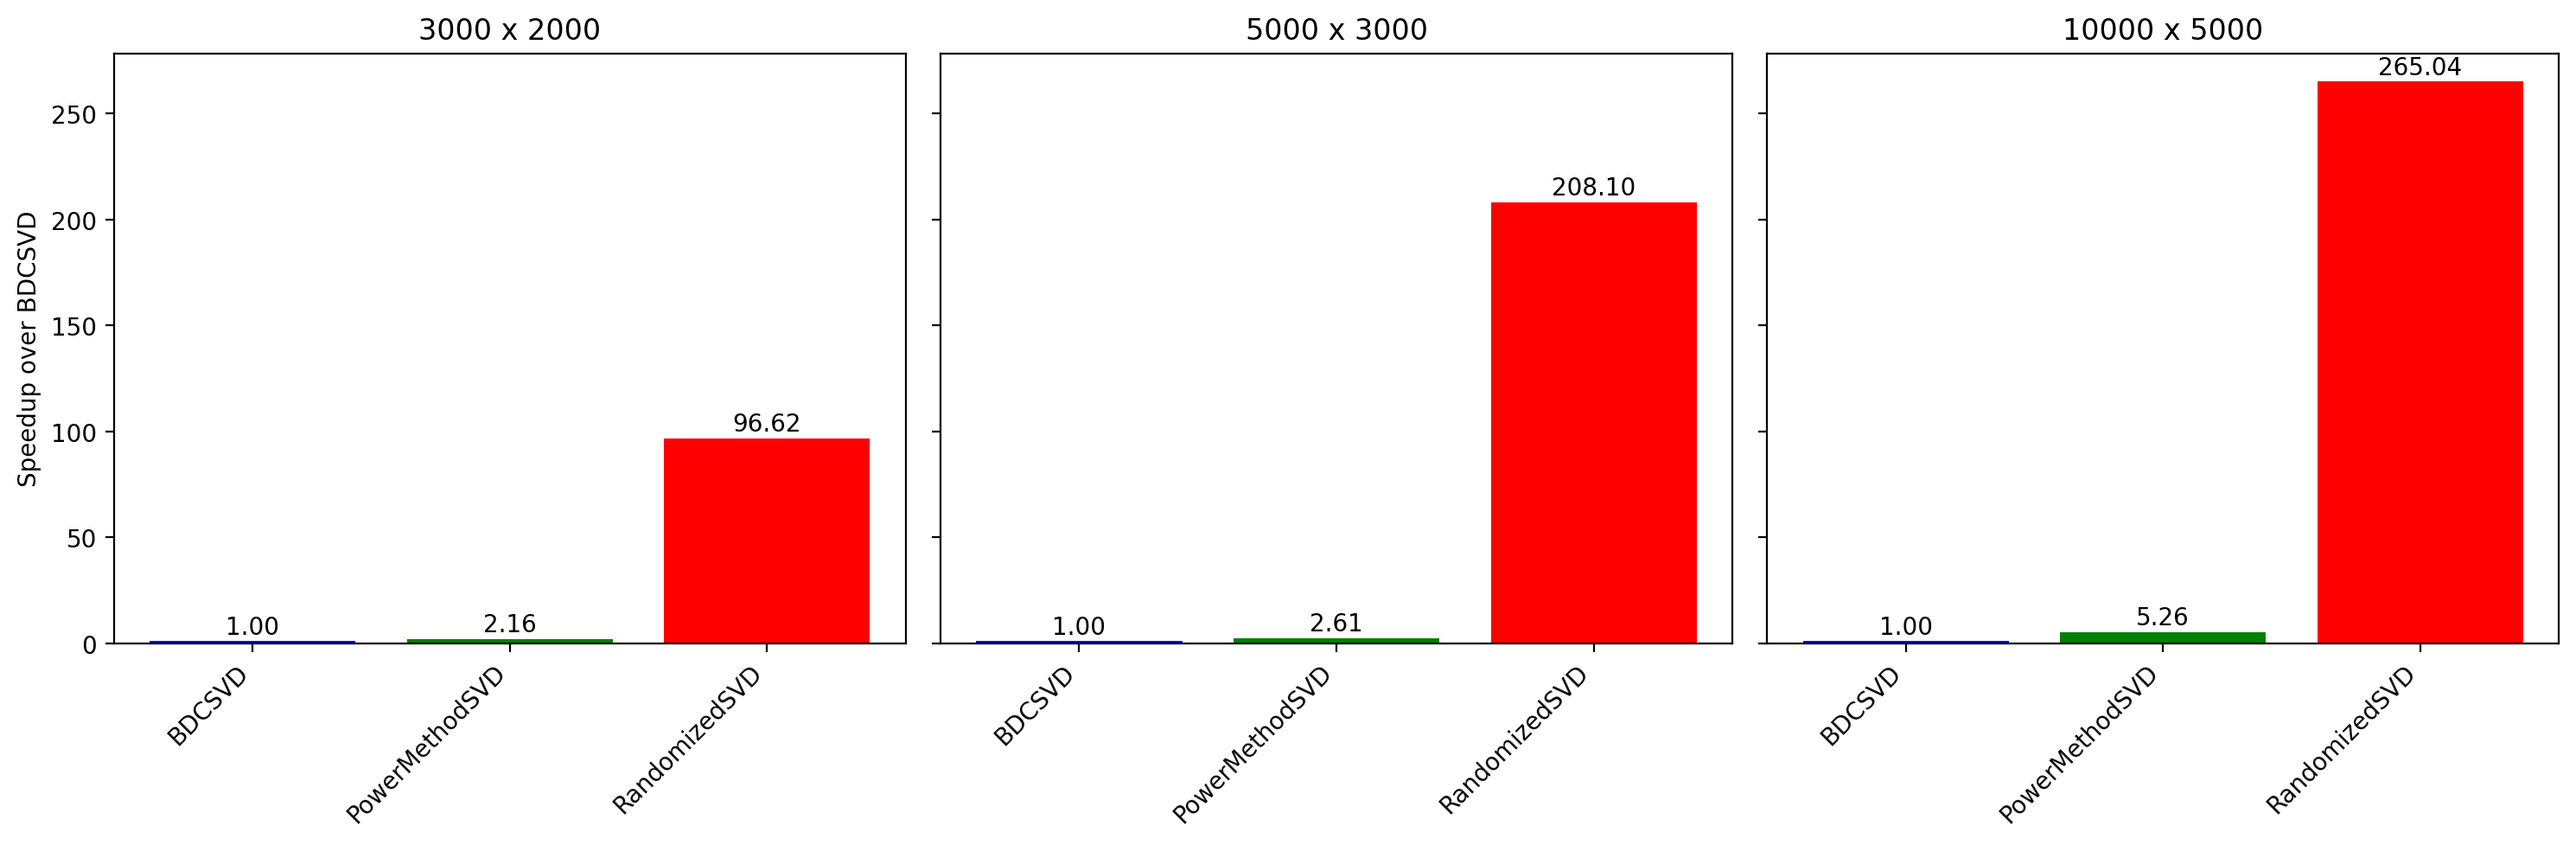
\includegraphics[width=\textwidth]{Images/speedup.png}
    \caption{Randomized SVD}
    \label{fig:speedup}
\end{figure}

%-----------------------------------------------------------------------------
% EQUATIONS
%-----------------------------------------------------------------------------
\section{Randomized Linear Algebra}
Random Linear Algebra is a branch of mathematics that combines principles from linear algebra with techniques from probability and statistics to analyze and solve problems involving large-scale or high-dimensional data. The base idea is to introduce \textbf{randomness} into computations to make algorithms faster, simpler, more efficient, more scalable, or more robust while maintaining accurate approximations of the desired results. This is needed because traditional linear algebra techniques can become computationally expensive for large datasets, such as those encountered in machine learning, data science, and numerical simulations. Randomized algorithms help mitigate these challenges by:
\begin{itemize}
    \item Reducing computation complexity
    \item Lowering memory requirements
    \item Allowing for parallelization and distributed computing
\end{itemize}



The main techniques used are:
\begin{itemize}
    \item \textbf{Randomized Sampling}: instead of processing an entire matrix, Randomized Linear Algebra uses random sampling to approximate matrix operations. For example by:
          \begin{itemize}
              \item \textit{Row/column sampling}: selecting a subset of rows or columns from a matrix based on a probability distribution to approximate its structure.
              \item \textit{Sketching}: compressing a large matrix into a smaller one ("sketch matrix") while preserving key properties, such as norms or singular values.
          \end{itemize}
    \item \textbf{Low-Rank Approximation}: many large matrices encountered in practice are approximately low-rank, meaning their significant information can be captured by a smaller number of dimensions. Randomized techniques are used to compute these approximations efficiently:
          \begin{itemize}
              \item \textit{Randomized SVD (Singular Value Decomposition)}: Approximating the singular values and vectors using random projections.
              \item \textit{CUR Decomposition}: representing a matrix using a subset of its actual rows (C) and columns (R), and a smaller core matrix (U).
          \end{itemize}
    \item \textbf{Random Projections}: high-dimensional data can be projected into a lower-dimensional space using random matrices, such as Gaussian random matrices and Sparse random matrices.
    \item \textbf{Montecarlo methods}: randomized algorithms often rely on Monte Carlo methods to provide probabilistic guarantees about the accuracy of approximations. For example, the probability of achieving a given approximation error is often a parameter of the algorithm.
    \item \textbf{Stochastic Iterative Methods}: iterative solvers for linear systems, such as gradient descent, can be randomized by incorporating stochastic components, which often improves convergence rates or reduces computational cost in large-scale problems.
\end{itemize}

\subsection{Challenges}
The main challenges that arise when using Randomized Linear Algebra are





\section{Randomized Singular Value Decomposition}

\subsection{QR Factorization}
The Givens Rotation $Q R$ decomposition is a method for decomposing a matrix $A$ into an orthogonal matrix $Q$ and an upper triangular matrix $R$, such that:
\[
    A = Q R
\]
A Givens rotation matrix is used to zero out specific elements of a matrix. For two elements $a$ and $b$, the Givens rotation coefficients $c$ and $s$ are calculated such that:
\[
    \begin{bmatrix}
        c  & s \\
        -s & c
    \end{bmatrix}
    \begin{bmatrix}
        a \\
        b
    \end{bmatrix}
    =
    \begin{bmatrix}
        r \\
        0
    \end{bmatrix}
\]
where $r = \sqrt{a^2 + b^2}$. The Givens rotation matrix is then used to zero out the element $b$ by multiplying the matrix from the left:
\[
    \begin{bmatrix}
        c  & s \\
        -s & c
    \end{bmatrix}
    \begin{bmatrix}
        a & b \\
        c & d
    \end{bmatrix}
    =
    \begin{bmatrix}
        r & 0  \\
        0 & d'
    \end{bmatrix}
\]
where $d' = c d - s b$. The Givens rotation matrix is a simple and efficient way to perform QR decomposition, especially for sparse matrices. The pseudocode for the Givens rotation QR decomposition is shown in Algorithm \ref{alg:givens}.

\subsection{Singular Value Decompoition using Power Method}
The singular value decomposition (SVD) is a fundamental matrix decomposition method that decomposes a matrix $A$ into three matrices $U$, $\Sigma$, and $V$ such that:
\[
    A = U \Sigma V^T
\]
where $U$ and $V$ are orthogonal matrices and $\Sigma$ is a diagonal matrix with the singular values of $A$. The SVD is widely used in various applications, including dimensionality reduction, data compression, and machine learning. The power method is an iterative algorithm that can be used to compute the singular values and vectors of a matrix. The power method works by repeatedly multiplying the matrix by a vector and normalizing the result. The pseudocode for the power method SVD is shown in Algorithm \ref{alg:power}.

\subsection{Algorithm Description}
Let $A \in \mathbb{R}^{m \times n}$ be a matrix of low rank, and $m \ge n$.
In the following, we seek the near-optimal low-rank approximation of the form
\[
    A \approx U_k \Sigma_k V_k^T
\]
where $k$ denotes the target rank. Instead of computing the singular value decomposition directly, we embed the SVD into the probabilistic framework. The principal concept is sketched in Figure \ref{fig:rSVD}.

\begin{figure}[H]
    \centering
    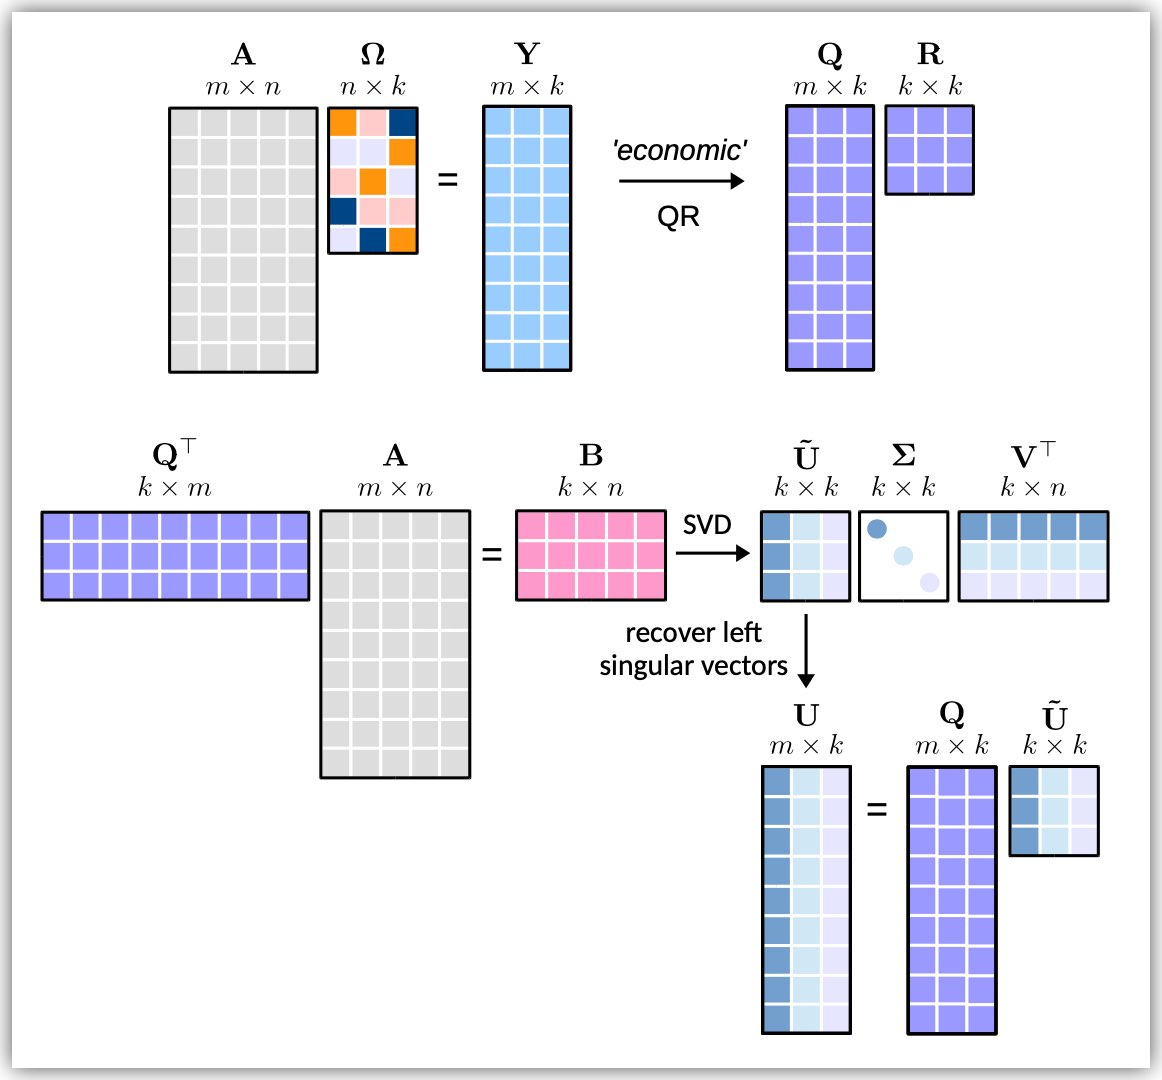
\includegraphics[height=0.3\textheight]{Images/rSVD.jpg}
    \caption{Randomized SVD \cite{erichsonRandomizedMatrixDecompositions2019}}
    \label{fig:rSVD}
\end{figure}

\subsection{Optimization technique}

\section{Applications}
In this section, we present some useful applications of the RandomizedSVD algorithm.
\subsection{Image Compression}
\subsubsection{Code Explanation}
\subsubsection{Results Analysis}



\subsection{Handwritten Numbers Recognition}
We implemented a handwritten digit recognition system using the MNIST dataset and our RandomizedSVD algorithm for dimensionality reduction. The system demonstrates how dimensionality reduction can be effectively used for classification tasks while maintaining high accuracy.

\subsubsection{Implementation Details}
The implementation consists of several key components:

\begin{itemize}
    \item \textbf{Data Loading}: The \texttt{MNISTLoader} class handles loading and preprocessing of the MNIST dataset, converting the binary data into Eigen matrices and normalizing pixel values to [0,1].
    
    \item \textbf{Dimensionality Reduction}: We use PCA with RandomizedSVD to reduce the dimension of the input images (784 dimensions) to a lower-dimensional space (2-256 components in our tests).
    
    \item \textbf{Classification}: The system uses a simple nearest neighbor classifier in the reduced space to predict digits.
\end{itemize}

The core algorithm workflow is:

\begin{enumerate}
    \item Center the data by subtracting the mean
    \item Project the data to a lower-dimensional space using PCA
    \item For prediction, project new images into the same space and find the nearest neighbor
\end{enumerate}

\subsubsection{Results Analysis}
We conducted extensive testing using 10,000 training images and 1,000 test images from the MNIST dataset. The results for different numbers of principal components are shown in Table \ref{table:mnist_accuracy}.

\begin{table}[H]
    \centering
    \begin{tabular}{|c|c|}
        \hline
        \rowcolor{bluePoli!40}
        \textbf{Number of Components} & \textbf{Accuracy} \T\B \\
        \hline
        2 & 37.9\% \T\B \\
        4 & 58.1\% \T\B \\
        8 & 85.1\% \T\B \\
        16 & 92.3\% \T\B \\
        32 & 93.7\% \T\B \\
        64 & 93.3\% \T\B \\
        128 & 93.1\% \T\B \\
        256 & 92.7\% \B \\
        \hline
    \end{tabular}
    \caption{Recognition accuracy with different numbers of principal components}
    \label{table:mnist_accuracy}
\end{table}

Key observations from the results:

\begin{itemize}
    \item \textbf{Rapid Improvement}: The accuracy improves dramatically from 37.9\% with 2 components to 85.1\% with just 8 components, showing that even a small number of carefully chosen components can capture significant discriminative information.
    
    \item \textbf{Optimal Range}: The accuracy peaks at 93.7\% with 32 components, suggesting this is the optimal trade-off between dimensionality reduction and information preservation for this task.
    
    \item \textbf{Diminishing Returns}: Beyond 32 components, the accuracy slightly decreases, indicating that additional components may be introducing noise rather than useful information.
\end{itemize}

We also tested the system on individual images, successfully recognizing test digits (e.g., correctly identifying a test image of the digit "6"). This demonstrates the practical applicability of our implementation for real-world digit recognition tasks.

The results show that our RandomizedSVD-based approach can achieve high accuracy while significantly reducing the dimensionality of the input data (from 784 to just 32 dimensions in the optimal case). This reduction leads to faster computation and lower memory requirements while maintaining excellent recognition performance.

\subsection{Principal Component Analysis (PCA)}
\subsubsection{Code Explanation}
\subsubsection{Results Analysis}


\section{CUR Decomposition}
\subsection{Algorithm}
\subsubsection{Code Explanation}
\subsection{Results Analysis}
\section{Conclusion}
\subsection{Possible Further Applications}
Present some possible further applications or possible further development of the ones presented.

\section{Bibliography and citations}

\section{Appendix - Group Work Organization}
Here explain the contributions from each member of the group.\\
\textbf{FROM HERE ON IT'S JUST CODE EXAMPLES}
\section{Equations}
\label{sec:eqs}
This section gives some examples of writing mathematical equations in your thesis.

Maxwell's equations read:
\begin{subequations}
    \label{eq:maxwell}
    \begin{align}[left=\empheqlbrace]
        \nabla\cdot \bm{D}                                         & = \rho, \label{eq:maxwell1}   \\
        \nabla \times \bm{E} +  \frac{\partial \bm{B}}{\partial t} & = \bm{0}, \label{eq:maxwell2} \\
        \nabla\cdot \bm{B}                                         & = 0, \label{eq:maxwell3}      \\
        \nabla \times \bm{H} - \frac{\partial \bm{D}}{\partial t}  & = \bm{J}. \label{eq:maxwell4}
    \end{align}
\end{subequations}

Equation~\eqref{eq:maxwell} is automatically labeled by \texttt{cleveref},
as well as Equation~\eqref{eq:maxwell1} and Equation~\eqref{eq:maxwell3}.
Thanks to the \verb|cleveref| package, there is no need to use \verb|\eqref|.
Equations have to be numbered only if they are referenced in the text.

Equations~\eqref{eq:maxwell_multilabels1}, \eqref{eq:maxwell_multilabels2}, \eqref{eq:maxwell_multilabels3}, and \eqref{eq:maxwell_multilabels4} show again Maxwell's equations without brace:
\begin{align}
    \nabla\cdot \bm{D}                                         & = \rho, \label{eq:maxwell_multilabels1}   \\
    \nabla \times \bm{E} +  \frac{\partial \bm{B}}{\partial t} & = \bm{0}, \label{eq:maxwell_multilabels2} \\
    \nabla\cdot \bm{B}                                         & = 0, \label{eq:maxwell_multilabels3}      \\
    \nabla \times \bm{H} - \frac{\partial \bm{D}}{\partial t}  & = \bm{J} \label{eq:maxwell_multilabels4}.
\end{align}

Equation~\eqref{eq:maxwell_singlelabel} is the same as before,
but with just one label:
\begin{equation}
    \label{eq:maxwell_singlelabel}
    \left\{
    \begin{aligned}
        \nabla\cdot \bm{D}                                         & = \rho,   \\
        \nabla \times \bm{E} +  \frac{\partial \bm{B}}{\partial t} & = \bm{0}, \\
        \nabla\cdot \bm{B}                                         & = 0,      \\
        \nabla \times \bm{H} - \frac{\partial \bm{D}}{\partial t}  & = \bm{J}.
    \end{aligned}
    \right.
\end{equation}

%-----------------------------------------------------------------------------
% FIGURES, TABLES AND ALGORITHMS
%-----------------------------------------------------------------------------
\section{Figures, Tables and Algorithms}

Figures, Tables and Algorithms have to contain a Caption that describes their content, and have to be properly referred in the text.

\subsection{Figures}
\label{subsec:figures}

For including pictures in your text you can use \texttt{TikZ} for high-quality hand-made figures \cite{tikz},
or just include them with the command
\begin{verbatim}
\includegraphics[options]{filename.xxx}
\end{verbatim}
Here xxx is the correct format, e.g.  \verb|.png|, \verb|.jpg|, \verb|.eps|, \dots.

\begin{figure}[H]
    \centering
    
\includegraphics[width=0.3\textwidth]{logo_polimi_scritta.eps}
    \caption{Caption of the Figure.}
    \label{fig:quadtree}
\end{figure}

Thanks to the \texttt{\textbackslash subfloat} command, a single figure, such as Figure~\ref{fig:quadtree},
can contain multiple sub-figures with their own caption and label, e.g. Figure~\ref{fig:polimi_logo1} and Figure~\ref{fig:polimi_logo2}.

\begin{figure}[H]
    \centering
    \subfloat[One PoliMi logo.\label{fig:polimi_logo1}]{
        
\includegraphics[scale=0.5]{Images/logo_polimi_scritta.eps}
    }
    \quad
    \subfloat[Another one PoliMi logo.\label{fig:polimi_logo2}]{
        
\includegraphics[scale=0.5]{Images/logo_polimi_scritta2.eps}
    }
    \caption[]{Caption of the Figure.}
    \label{fig:quadtree2}
\end{figure}

\subsection{Tables}
\label{subsec:tables}

Within the environments \texttt{table} and  \texttt{tabular} you can create very fancy tables as the one shown in Table~\ref{table:example}.

\begin{table}[H]
    \caption*{\textbf{Example of Table (optional)}}
    \centering
    \begin{tabular}{|p{3em} c c c |}
        \hline
        \rowcolor{bluePoli!40}
                      & \textbf{column1} & \textbf{column2} & \textbf{column3} \T\B \\
        \hline \hline
        \textbf{row1} & 1                & 2                & 3 \T\B                \\
        \textbf{row2} & $\alpha$         & $\beta$          & $\gamma$ \T\B         \\
        \textbf{row3} & alpha            & beta             & gamma \B              \\
        \hline
    \end{tabular}
    \\[10pt]
    \caption{Caption of the Table.}
    \label{table:example}
\end{table}

You can also consider to highlight selected columns or rows in order to make tables more readable.
Moreover, with the use of \texttt{table*} and the option \texttt{bp} it is possible to align them at the bottom of the page. One example is presented in Table~\ref{table:exampleC}.

\begin{table*}[bp]
    \centering
    \begin{tabular}{|p{3em} | c | c | c | c | c | c|}
        \hline
        %    \rowcolor{bluePoli!40}
                      & \textbf{column1} & \textbf{column2} & \textbf{column3} & \textbf{column4} & \textbf{column5} & \textbf{column6} \T\B \\
        \hline \hline
        \textbf{row1} & 1                & 2                & 3                & 4                & 5                & 6 \T\B                \\
        \textbf{row2} & a                & b                & c                & d                & e                & f \T\B                \\
        \textbf{row3} & $\alpha$         & $\beta$          & $\gamma$         & $\delta$         & $\phi$           & $\omega$ \T\B         \\
        \textbf{row4} & alpha            & beta             & gamma            & delta            & phi              & omega \B              \\
        \hline
    \end{tabular}
    \\[10pt]
    \caption{Highlighting the columns}
    \label{table:exampleC}
\end{table*}

\subsection{Algorithms}
\label{subsec:algorithms}

Pseudo-algorithms can be written in \LaTeX{} with the \texttt{algorithm} and \texttt{algorithmic} packages.
An example is shown in Algorithm~\ref{alg:var}.
\begin{algorithm}[H]
    \label{alg:example}
    \caption{Name of the Algorithm}
    \label{alg:var}
    \label{protocol1}
    \begin{algorithmic}[1]
        \STATE Initial instructions
        \FOR{$for-condition$}
        \STATE{Some instructions}
        \IF{$if-condition$}
        \STATE{Some other instructions}
        \ENDIF
        \ENDFOR
        \WHILE{$while-condition$}
        \STATE{Some further instructions}
        \ENDWHILE
        \STATE Final instructions
    \end{algorithmic}
\end{algorithm}

\section{Some further useful suggestions}

Theorems have to be formatted as follows:
\begin{theorem}
    \label{a_theorem}
    Write here your theorem.
\end{theorem}
\textit{Proof.} If useful you can report here the proof.
\vspace{0.3cm} % Insert vertical space

Propositions have to be formatted as follows:
\begin{proposition}
    Write here your proposition.
\end{proposition}
\vspace{0.3cm} % Insert vertical space

How to insert itemized lists:
\begin{itemize}
    \item first item;
    \item second item.
\end{itemize}
How to write numbered lists:
\begin{enumerate}
    \item first item;
    \item second item.
\end{enumerate}

\section{Use of copyrighted material}

Each student is responsible for obtaining copyright permissions, if necessary, to include published material in the thesis.
This applies typically to third-party material published by someone else.

\section{Plagiarism}

You have to be sure to respect the rules on Copyright and avoid an involuntary plagiarism.
It is allowed to take other persons' ideas only if the author and his original work are clearly mentioned.
As stated in the Code of Ethics and Conduct, Politecnico di Milano \textit{promotes the integrity of research,
    condemns manipulation and the infringement of intellectual property}, and gives opportunity to all those
who carry out research activities to have an adequate training on ethical conduct and integrity while doing research.
To be sure to respect the copyright rules, read the guides on Copyright legislation and citation styles available
at:
\begin{verbatim}
https://www.biblio.polimi.it/en/tools/courses-and-tutorials
\end{verbatim}
You can also attend the courses which are periodically organized on "Bibliographic citations and bibliography management".

%-----------------------------------------------------------------------------
% CONCLUSION
%-----------------------------------------------------------------------------
\section{Conclusions}
\color{black}
A final section containing the main conclusions of your research/study
and possible future developments of your work have to be inserted in the section ``Conclusions''.

\section{Bibliography and citations}
Your thesis must contain a suitable Bibliography which lists all the sources consulted on developing the work.
The list of references is placed at the end of the manuscript after the chapter containing the conclusions.
It is suggested to use the BibTeX package and save the bibliographic references in the file \verb|bibliography.bib|.
This is indeed a database containing all the information about the references. To cite in your manuscript, use the \verb|\cite{}| command as follows:
\\
\textit{Here is how you cite bibliography entries: \cite{knuth74}, or multiple ones at once: \cite{knuth92,lamport94}}.
\\
The bibliography and list of references are generated automatically by running BibTeX \cite{bibtex}.

%-----------------------------------------------------------------------------
% BIBLIOGRAPHY
%-----------------------------------------------------------------------------
\bibliography{bibliography.bib}

\appendix
\section{Appendix A}
If you need to include an appendix to support the research in your thesis, you can place it at the end of the manuscript.
An appendix contains supplementary material (figures, tables, data, codes, mathematical proofs, surveys, \dots)
which supplement the main results contained in the previous sections.

\section{Appendix B}
It may be necessary to include another appendix to better organize the presentation of supplementary material.

%%%%%%%%%%%%%%%%%%%%%%%%%%%%%%%%%%%%%%%%%%%%%%%%%%%%%%%%%%%%%%
%%     ABSTRACT IN ITALIAN LANGUAGE AND ACKNOWLEDGMENTS     %%
%%%%%%%%%%%%%%%%%%%%%%%%%%%%%%%%%%%%%%%%%%%%%%%%%%%%%%%%%%%%%%
\cleardoublepage

%-----------------------------------------------------------------------------
% SOMMARIO
%-----------------------------------------------------------------------------
\section*{Abstract in lingua italiana}
Qui va l'Abstract in lingua italiana della tesi seguito dalla lista di parole chiave.
\vspace{15pt}
\begin{tcolorbox}[arc=0pt, boxrule=0pt, colback=bluePoli!60, width=\textwidth, colupper=white]
    \textbf{Parole chiave:} qui, le parole chiave, della tesi, in italiano
\end{tcolorbox}

%-----------------------------------------------------------------------------
% ACKNOWLEDGEMENTS
%-----------------------------------------------------------------------------
\section*{Acknowledgements}
Here you might want to acknowledge someone.

%-------------------------------------------------------------------------
%	END OF YOUR DOCUMENT
%-------------------------------------------------------------------------
\end{document}